\documentclass[11pt,a4paper,landscape]{article}
%\usepackage{array}
\usepackage{german}
\usepackage[latin1]{inputenc}
\usepackage[final]{epsfig}
%\usepackage{array}
\usepackage{tabularx}
\usepackage{times}

\pagestyle{empty}

\setlength{\oddsidemargin}{0.0cm}
\setlength{\textwidth}{27.0cm}

\setlength{\topmargin}{0.0cm}
\setlength{\headheight}{0.0cm}
\setlength{\headsep}{0.0cm}
\setlength{\topskip}{0.0cm}
\setlength{\textheight}{20cm}

\setlength{\voffset}{-1.8cm}
\setlength{\hoffset}{-1.8cm}


\newcommand{\LI}{\setlength{\arrayrulewidth}{0.4mm}}
\newcommand{\li}{\setlength{\arrayrulewidth}{0.2mm}}
\setlength{\doublerulesep}{0mm}

\begin{document}
\newsavebox{\ESchwert}    
\newsavebox{\Stichwaffe}  
\newsavebox{\ESchlagwaffe}
\newsavebox{\Spiesswaffe}
\newsavebox{\ZSchwert}
\newsavebox{\ZSchlagwaffe}
\newsavebox{\Stangenwaffe}
\newsavebox{\Kettenwaffe} 
\newsavebox{\Bogen}       
\newsavebox{\Armbrust}    
\newsavebox{\Schleuder}   
\newsavebox{\Wurfspiess}  
\newsavebox{\WSchlagwaffe}
\newsavebox{\Schilde}
%%
\newsavebox{\Magierstab}
\newsavebox{\waffenlos} 
\newsavebox{\Blasrohr}  
\newsavebox{\Wurfpfeil} 
\newsavebox{\Wurfmesser}
\newsavebox{\Wurfstern} 
\newsavebox{\Kampfstab} 
\newsavebox{\Parierdolch}
\newsavebox{\Bola}
\newsavebox{\Netz}
\newsavebox{\Peitsche}
\newsavebox{\Lasso}   
%\input{midgard_tmp_latexwertedef}
\input{midgard_tmp_latexwerte}
\parbox{10cm}{
\epsfig{width=10cm,angle=0,file=/usr/local/share/midgard/drache.ps}}
\parbox[][][c]{7cm}{
\LI
  \begin{tabularx}{7.0cm}{|c|X|}\hline
\makebox[1.1cm]{Figur}&\resizebox*{4.5cm}{2ex}{\namecharakter}\\\hline
  \end{tabularx}

\vspace{2mm}\li
  \begin{tabularx}{7.0cm}{|c|X|}\hline
\makebox[1.1cm]{Spieler}&{\namespieler}\\\hline
  \end{tabularx}
}
\parbox{10cm}{
\epsfig{width=10cm,angle=0,file=/usr/local/share/midgard/dracher.ps}}

\vspace*{2ex}
\begin{minipage}[t]{13cm}
\LI
  \begin{tabular}[t]{|c|l|}\hline
\makebox[1.1cm]{\rule[-1.4ex]{0cm}{4ex}Typ}&\makebox[2.2cm]{\resizebox*{2.2cm}{2ex}{{\typ}}}\\\hline
  \end{tabular}
\hfill 
\li
  \begin{tabular}[t]{|c|l|}\hline
\makebox[1.1cm]{\rule[-1.4ex]{0cm}{4ex}\parbox[][][c]{1.1cm}{\renewcommand{\baselinestretch}{0}
\footnotesize Speziali"-sierung}}&\makebox[2.5cm]{{\spezialisierung}}\\\hline
  \end{tabular}\renewcommand{\baselinestretch}{1}
\hfill 
\LI
  \begin{tabular}[t]{|c|l|}\hline
\makebox[1.05cm]{\rule[-1.4ex]{0cm}{4ex}Grad}&\makebox[1.5cm]{{\grad}}\\\hline
  \end{tabular}

\vspace{2ex}
\li
  \begin{tabular}{|c|l|}\hline
\makebox[1.1cm]{\rule[-1.4ex]{0cm}{4ex}\small Herkunft}&\makebox[2.2cm]{\resizebox*{2cm}{2ex}{{\herkunft}}}\\\hline
  \end{tabular}
\hfill
\li
  \begin{tabular}{|c|l|}\hline
%\makebox[1.1cm]{\rule[-1.4ex]{0cm}{4ex}Glaube}&\makebox[2.5cm]{\resizebox*{2.5cm}{2ex}{\glaube}}\\\hline
\makebox[1.1cm]{\rule[-1.4ex]{0cm}{4ex}Glaube}&\makebox[2.5cm]{\glaube}\\\hline
  \end{tabular}
\hfill
\li
  \begin{tabular}{|c|l|}\hline
\makebox[1.1cm]{\rule[-1.4ex]{0cm}{4ex}Stand}&\makebox[1.5cm]{\resizebox*{1.5cm}{2ex}{{\stand}}}\\\hline
  \end{tabular}

\vspace{2ex}
{\small
\begin{tabular}{|c|l|}\hline
Alter&\makebox[0.8cm]{{\alter}}\\\hline
\end{tabular}\hfill
\begin{tabular}{|c|l|}\hline
Gestalt&\makebox[0.8cm]{\resizebox*{0.7cm}{2ex}{{\gestalt}}}\\\hline
\end{tabular}\hfill
\begin{tabular}{|c|l|}\hline
Gewicht&\makebox[0.8cm]{{\gewicht}}\\\hline
\end{tabular}\hfill
\begin{tabular}{|c|l|}\hline
K�rpergr��e&\makebox[0.8cm]{{\koerpergroesse}}\\\hline
\end{tabular}

\vspace{2ex}
\renewcommand{\arraystretch}{0.9}
\begin{tabularx}{13cm}{|c|X|}\hline
Berufe&{\beruf}\\\hline
%Sprachen&\\\hline
%Schriften&\\\hline
\raisebox{-0.3ex}[0.3ex]{weitere}&\\
\raisebox{0.3ex}[-0.3ex]{Merkmale}\rule[-1ex]{0ex}{3.3ex}&\\\hline
\end{tabularx}\renewcommand{\arraystretch}{1}
}

\vspace{2ex}
\normalsize
\LI
\begin{tabular}{|c|c|}\hline
\makebox[0.6cm]{St}&\makebox[0.6cm]{{\st}}\\\hline
\end{tabular}\hfill
\begin{tabular}{|c|c|}\hline
\makebox[0.6cm]{Ge}&\makebox[0.6cm]{{\gee}}\\\hline
\end{tabular}\hfill
\begin{tabular}{|c|c|}\hline
\makebox[0.6cm]{Ko}&\makebox[0.6cm]{{\ko}}\\\hline
\end{tabular}\hfill
\begin{tabular}{|c|c|}\hline
\makebox[0.6cm]{In}&\makebox[0.6cm]{{\inn}}\\\hline
\end{tabular}\hfill
\begin{tabular}{|c|c|}\hline
\makebox[0.6cm]{Zt}&\makebox[0.6cm]{{\zt}}\\\hline
\end{tabular}

\vspace{2ex}
\li
\begin{tabular}{|c|c|}\hline
\makebox[0.6cm]{Au}&\makebox[0.6cm]{{\au}}\\\hline
\end{tabular}\hfill
\begin{tabular}{|c|c|}\hline
\makebox[0.6cm]{pA}&\makebox[0.6cm]{{\pa}}\\\hline
\end{tabular}\hfill
\begin{tabular}{|c|c|}\hline
\makebox[0.6cm]{Sb}&\makebox[0.6cm]{{\sbb}}\\\hline
\end{tabular}\hfill
\begin{tabular}{|c|c|}\hline
\makebox[0.6cm]{RW}&\makebox[0.6cm]{{\rw}}\\\hline
\end{tabular}\hfill
\begin{tabular}{|c|c|}\hline
\makebox[0.6cm]{HGW}&\makebox[0.6cm]{{\hgw}}\\\hline
\end{tabular}

\vspace{2ex}
\LI
\begin{tabular}{|c|c|}\hline
\makebox[0.6cm]{B}&\makebox[0.6cm]{{\bb}}\\\hline
\end{tabular}\hfill
\li
\begin{tabular}{|c|c|}\hline
\makebox[0.6cm]{KAW}&\makebox[0.6cm]{{\kaw}}\\\hline
\end{tabular}\hfill
\begin{tabular}{|c|c|}\hline
\makebox[0.6cm]{WLW}&\makebox[0.6cm]{{\wlw}}\\\hline
\end{tabular}\hfill
\begin{tabular}{|c|c|}\hline
\makebox[0.6cm]{\tiny LP-Basis}&\makebox[0.6cm]{{\lpbasis}}\\\hline
\end{tabular}\hfill
\begin{tabular}{|c|c|}\hline
\makebox[0.6cm]{}&\hspace*{0.6cm}\\\hline
\end{tabular}

\vspace{2ex}
{\footnotesize
\setlength{\tabcolsep}{-0.0135cm}
\begin{tabular*}{13cm}{|c|c|c|c|c||c|c|c||c|}
\multicolumn{9}{l}{\hspace*{1ex}pers�nliche Boni f�r}\\\hline
\makebox[1.44444cm]{\scriptsize Ausdauer}&\makebox[1.44444cm]{Schaden}&\makebox[1.44444cm]{Angriff}&\makebox[1.44444cm]{Abwehr}&\makebox[1.44444cm]{Zauber}&\makebox[1.44444cm]{psyZR}&\makebox[1.44444cm]{phsZR}&\makebox[1.44444cm]{phkZR}&\makebox[1.44444cm]{Gift TB}\\\hline
{\boau}&{\bosc}&{\boan}&{\boab}&{\boza}&{\bopsy}&{\bophs}&{\bophk}&{\bogi}\\\hline
\end{tabular*}
}

{\small
\begin{tabular}{|c|l|}\hline
Abwehr&\makebox[0.2cm]{{\abwehr}}\\\hline
\end{tabular}\hfill
\begin{tabular}{|c|l|}\hline
Zaubern&\makebox[0.2cm]{{\zauber}}\\\hline
\end{tabular}\hfill
{\setlength{\tabcolsep}{-0.0135cm}
\begin{tabular}{|c||c|c|c||c|}\hline
\footnotesize\hspace*{1ex}Resistenzen\hspace*{1ex}&\makebox[1.44444cm]{{\psy}}&\makebox[1.44444cm]{{\phs}}&\makebox[1.44444cm]{{\phk}}&\makebox[1.44444cm]{{\gift}}\\\hline
\end{tabular}}}

\vspace{2ex}\LI
\begin{tabularx}{13cm}{|p{0.5cm}|c|X|}\hline
\makebox[0.5cm]{LP}&\makebox[0.5cm]{{\lp}}&\\\hline
\makebox[0.5cm]{AP}&\makebox[0.5cm]{{\ap}}&\\\hline
\end{tabularx}

\li
\vspace*{3ex}
{\setlength{\tabcolsep}{1.4ex}
\scriptsize
\begin{tabular}{|c@{\LI\hspace*{1.4ex}\vline\hspace*{1.4ex}}c@{\LI\hspace*{1.4ex}\vline\hspace*{1.4ex}}c|c|c|c|} \hline
Datum&GFP&KEP&ZEP&AEP&Geld\\\hline\hline
&{\gfp}&&&&{\gold}\\\hline
&&&&&\\\hline
&&&&&\\\hline
&&&&&\\\hline
&&&&&\\\hline
&&&&&\\\hline
&&&&&\\\hline
&&&&&\\\hline
&&&&&\\\hline
&&&&&\\\hline
&&&&&\\\hline
&&&&&\\\hline
&&&&&\\\hline
&&&&&\\\hline
\end{tabular}
\hfill
\begin{tabular}{|p{2.4cm}|c|p{2.4cm}|}
  \hline
Sprache&&Schrift\\\hline\hline
{\spraa}&{\sprawa}&{\schra}\\\hline
{\sprab}&{\sprawb}&{\schrb}\\\hline
{\sprac}&{\sprawc}&{\schrc}\\\hline
{\sprad}&{\sprawd}&{\schrd}\\\hline
{\sprae}&{\sprawe}&{\schre}\\\hline
{\spraf}&{\sprawf}&{\schrf}\\\hline
{\sprag}&{\sprawg}&{\schrg}\\\hline
{\sprah}&{\sprawh}&{\schrh}\\\hline
{\sprai}&{\sprawi}&{\schri}\\\hline
{\spraj}&{\sprawj}&{\schrj}\\\hline
{\sprak}&{\sprawk}&{\schrk}\\\hline
{\spral}&{\sprawl}&{\schrl}\\\hline
{\spram}&{\sprawm}&{\schrm}\\\hline
{\spran}&{\sprawn}&{\schrn}\\\hline
\end{tabular} 
}
\end{minipage}
\hspace{3ex}
\begin{minipage}[t]{5.4cm}
\small
    \begin{tabular}[t]{|p{3cm}|p{0.5cm}|p{0.5cm}|}\hline
      \multicolumn{3}{|c|}{\small erlernte und angeborene}\\
      \multicolumn{3}{|c|}{\small F�higkeiten und Waffenfertigkeiten}\\[1ex]
      \normalsize Fertigkeit&\normalsize PP&\normalsize EW\\\hline\hline
\makebox[3cm][l]{{\ferta}}      &&\makebox[0.5cm]{{\werta}}\\\hline
\makebox[3cm][l]{{\fertb}}      &&\makebox[0.5cm]{{\wertb}}\\\hline
\makebox[3cm][l]{{\fertc}}      &&\makebox[0.5cm]{{\wertc}}\\\hline
\makebox[3cm][l]{{\fertd}}      &&\makebox[0.5cm]{{\wertd}}\\\hline
\makebox[3cm][l]{{\ferte}}      &&\makebox[0.5cm]{{\werte}}\\\hline
\makebox[3cm][l]{{\fertf}}      &&\makebox[0.5cm]{{\wertf}}\\\hline
\makebox[3cm][l]{{\fertg}}      &&\makebox[0.5cm]{{\wertg}}\\\hline
\makebox[3cm][l]{{\ferth}}      &&\makebox[0.5cm]{{\werth}}\\\hline
\makebox[3cm][l]{{\ferti}}      &&\makebox[0.5cm]{{\werti}}\\\hline
\makebox[3cm][l]{{\fertj}}      &&\makebox[0.5cm]{{\wertj}}\\\hline
\makebox[3cm][l]{{\fertk}}      &&\makebox[0.5cm]{{\wertk}}\\\hline
\makebox[3cm][l]{{\fertl}}      &&\makebox[0.5cm]{{\wertl}}\\\hline
\makebox[3cm][l]{{\fertm}}      &&\makebox[0.5cm]{{\wertm}}\\\hline
\makebox[3cm][l]{{\fertn}}      &&\makebox[0.5cm]{{\wertn}}\\\hline
\makebox[3cm][l]{{\ferto}}      &&\makebox[0.5cm]{{\werto}}\\\hline
\makebox[3cm][l]{{\fertp}}      &&\makebox[0.5cm]{{\wertp}}\\\hline
\makebox[3cm][l]{{\fertq}}      &&\makebox[0.5cm]{{\wertq}}\\\hline
\makebox[3cm][l]{{\fertr}}      &&\makebox[0.5cm]{{\wertr}}\\\hline
\makebox[3cm][l]{{\ferts}}      &&\makebox[0.5cm]{{\werts}}\\\hline
\makebox[3cm][l]{{\fertt}}      &&\makebox[0.5cm]{{\wertt}}\\\hline
\makebox[3cm][l]{{\fertu}}      &&\makebox[0.5cm]{{\wertu}}\\\hline
\makebox[3cm][l]{{\fertv}}      &&\makebox[0.5cm]{{\wertv}}\\\hline
\makebox[3cm][l]{{\fertw}}      &&\makebox[0.5cm]{{\wertw}}\\\hline
\makebox[3cm][l]{{\fertx}}      &&\makebox[0.5cm]{{\wertx}}\\\hline
\makebox[3cm][l]{{\ferty}}      &&\makebox[0.5cm]{{\werty}}\\\hline
\makebox[3cm][l]{{\fertz}}      &&\makebox[0.5cm]{{\wertz}}\\\hline
\makebox[3cm][l]{{\fertaa}}      &&\makebox[0.5cm]{{\wertaa}}\\\hline
\makebox[3cm][l]{{\fertab}}      &&\makebox[0.5cm]{{\wertab}}\\\hline
\makebox[3cm][l]{{\fertac}}      &&\makebox[0.5cm]{{\wertac}}\\\hline
\makebox[3cm][l]{{\fertad}}      &&\makebox[0.5cm]{{\wertad}}\\\hline
\makebox[3cm][l]{{\fertae}}      &&\makebox[0.5cm]{{\wertae}}\\\hline
\makebox[3cm][l]{{\fertaf}}      &&\makebox[0.5cm]{{\wertaf}}\\\hline
\makebox[3cm][l]{{\fertag}}      &&\makebox[0.5cm]{{\wertag}}\\\hline
\makebox[3cm][l]{{\fertah}}      &&\makebox[0.5cm]{{\wertah}}\\\hline
\makebox[3cm][l]{{\fertai}}      &&\makebox[0.5cm]{{\wertai}}\\\hline
\makebox[3cm][l]{{\fertaj}}      &&\makebox[0.5cm]{{\wertaj}}\\\hline
    \end{tabular}
\end{minipage}
\hspace{2ex}
%\fbox{
\begin{minipage}[t]{7.5cm}
\small
    \begin{tabular*}{7.5cm}[t]{||c|c|c||}\hline\hline
      \raisebox{-1ex}[2ex][0ex]{\LARGE Waffe}&\normalsize Erfolgswert&\footnotesize Angriffsrang(mod.)\\\cline{2-3}
      \raisebox{-0.2ex}[1ex][0.2ex]{\footnotesize (Reichweite)}&\normalsize\raisebox{-0.2ex}[1ex][0.2ex]{Schaden}&\footnotesize Abwehrmod.\\\hline\hline\hline
      waffenloser&{\waffeEy}&\waffeAy\\\cline{2-3}
      Kampf&{\waffeSy}&\waffeVy\\\hline\hline
      &{\waffeEa}&{\waffeAa}\\\cline{2-3}
      \raisebox{1.5ex}[-1.5ex]{\makebox[2cm][l]{{\waffea}}}&{\waffeSa}&{\waffeVa}\\\hline\hline
      &{\waffeEb}&{\waffeAb}\\\cline{2-3}
      \raisebox{1.5ex}[-1.5ex]{\makebox[2cm][l]{{\waffeb}}}&{\waffeSb}&{\waffeVb}\\\hline\hline
      &{\waffeEc}&{\waffeAc}\\\cline{2-3}
      \raisebox{1.5ex}[-1.5ex]{\makebox[2cm][l]{{\waffec}}}&{\waffeSc}&{\waffeVc}\\\hline\hline
      &{\waffeEd}&{\waffeAd}\\\cline{2-3}
      \raisebox{1.5ex}[-1.5ex]{\makebox[2cm][l]{{\waffed}}}&{\waffeSd}&{\waffeVd}\\\hline\hline
      &{\waffeEe}&{\waffeAe}\\\cline{2-3}
      \raisebox{1.5ex}[-1.5ex]{\makebox[2cm][l]{{\waffee}}}&{\waffeSe}&{\waffeVe}\\\hline\hline
      &{\waffeEf}&{\waffeAf}\\\cline{2-3}
      \raisebox{1.5ex}[-1.5ex]{\makebox[2cm][l]{{\waffef}}}&{\waffeSf}&{\waffeVf}\\\hline\hline
    \end{tabular*}
\parbox{7.5cm}{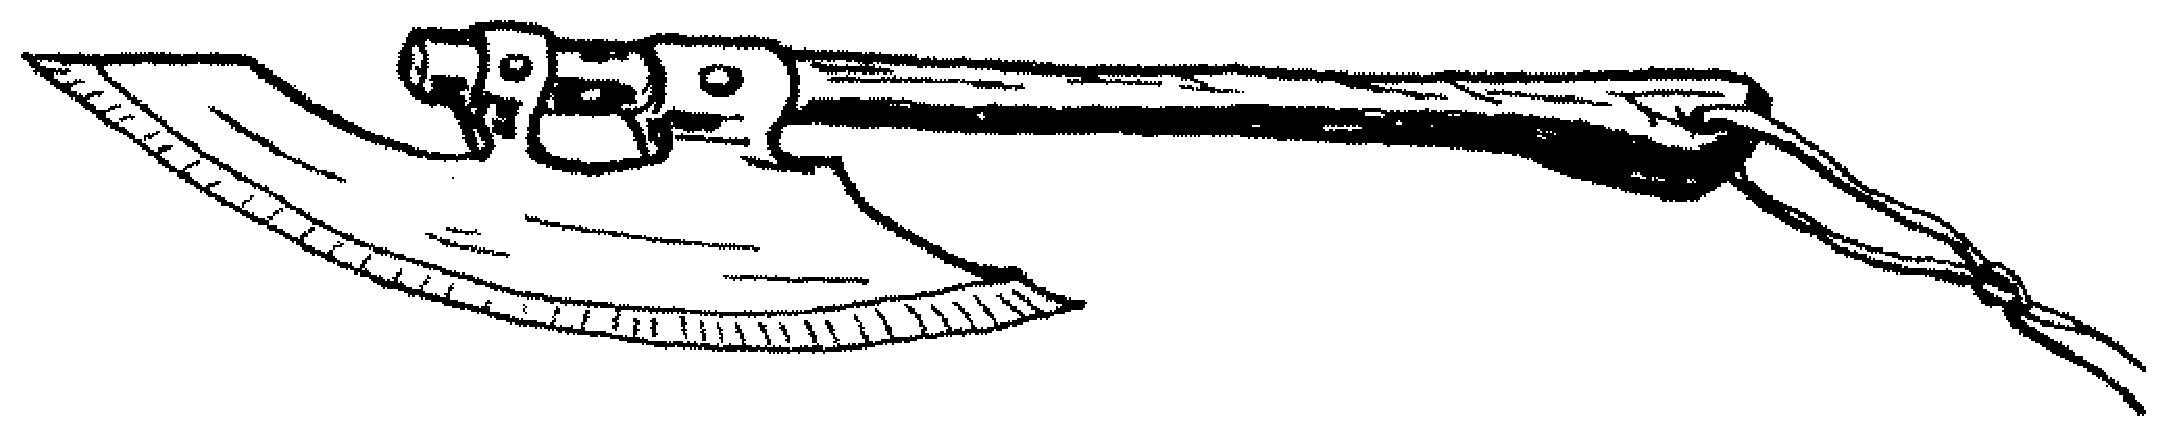
\epsfig{width=7.5cm,angle=0,file=/usr/local/share/midgard/axt1.ps}}
 \vspace*{2ex}
 \footnotesize
\parbox{7.7cm}
{
{\setlength{\tabcolsep}{1ex}\renewcommand{\arraystretch}{0.8}
    \begin{tabular}[b]{l|l|l|l|}
      \multicolumn{4}{l}{\small Grundkenntnisse in}\\\cline{2-2}\cline{4-4}
      ESchwert&{\usebox{\ESchwert}}&Kettenwaffe&\usebox{\Kettenwaffe}\\\cline{2-2}\cline{4-4}
      Stichwaffe&{\usebox{\Stichwaffe}}&Bogen&\usebox{\Bogen}\\\cline{2-2}\cline{4-4}
      ESchlagwaffe&{\usebox{\ESchlagwaffe}}&Armbrust&\usebox{\Armbrust}\\\cline{2-2}\cline{4-4}
      Spie�waffe&{\usebox{\Spiesswaffe}}&Schleuder&\usebox{\Schleuder}\\\cline{2-2}\cline{4-4}
      ZSchwert&{\usebox{\ZSchwert}}&Wurfspie�&\usebox{\Wurfspiess}\\\cline{2-2}\cline{4-4}
      ZSchlagwaffe&{\usebox{\ZSchlagwaffe}}&WSchlagwaffe&\usebox{\WSchlagwaffe}\\\cline{2-2}\cline{4-4}
      Stangenwaffe&{\usebox{\Stangenwaffe}}&Schild&\usebox{\Schilde}\\\cline{2-2}\cline{4-4}
    \end{tabular}}
\hfill
\LI
\scriptsize
{\setlength{\tabcolsep}{0.2ex}
    \begin{tabular}[b]{|c|c|}\hline
      R�stungs-&auf LP\\
      klasse&Verlust\\\hline
%      \rule{0ex}{0ex}&\\\hline
      {\ruestung}&{\ruestunglp}\\\hline
      \multicolumn{2}{c}{}\\\hline
      &mit Vert.\\
      \raisebox{1.5ex}[-1.5ex]{Abwehr}&Waffe\\\hline
       \rule{0ex}{0ex}{\abwehrfinal}&\\\hline
    \end{tabular}
}
}
\vspace{2ex}
{\renewcommand{\arraystretch}{0.7}
\begin{tabularx}{7.5cm}{lrXlr}
\multicolumn{5}{c}{\small Universelle Fertigkeiten}\\[1ex]
Balancieren&+8&&Schleichen&+1\\
Beredsamkeit&+3&&Schlittenfahren&+3\\
Beschatten&+3&&Schl�sser �ffnen&+0\\
Bet�uben&+6&&Schwimmen&+3\\
Fallen&+8&&Seilkunst&+4\\
Fallen entdecken&+0&&Springen&+8\\
Fallen entsch�rfen&+0&&Spurenlesen&+0\\
Fallenstellen&+1&&Stehlen&+3\\
Fangen&+8&&Tarnen&+1\\
Geheimmech. �ffnen&+1&&Tauchen&+9\\
Gel�ndelauf&+8&&�berleben&+6\\
Horchen&+2&&Verf�hren&+3\\
Kanufahren&+3&&Verh�ren&+3\\
Klettern&+8&&Verkleiden&+5\\
Landeskunde&+6&&Wagenlenken&+3\\
Meucheln&+0&&Wahrnehmung&+2\\
Reiten&+5&&Winden&+0\\
Rudern&+3&&&\\
\end{tabularx}}
\end{minipage}
%}
\end{document}


%%% Local Variables: 
%%% mode: latex
%%% TeX-master: t
%%% End: 
